\documentclass{article}

\usepackage{color,amsmath,amssymb,graphicx,fancyhdr,amsfonts,amsthm,verbatim,bbold,environ}
\usepackage{hyperref}
\usepackage{mkolar_definitions}
\usepackage{multirow}
\usepackage{diagbox}
\usepackage{longtable,booktabs}
\usepackage[left=2cm,top=2cm,right=2cm]{geometry}
\usepackage{listings}
% \numberwithin{algorithm}{section}


\newcommand{\tightlist}{%
  \setlength{\itemsep}{0pt}\setlength{\parskip}{0pt}}


%%%%%%%%%%%%%%%%%%%%%%%%%%%%%
\newcommand{\tta}{\theta}
\newcommand{\lag}{\left\langle}
\newcommand{\rag}{\right\rangle}
\newcommand{\lnorm}{\left\|}
\newcommand{\rnorm}{\right\|}
%%%%%%%%%%%%%%%%%%%%%%%%%%%%%
\usepackage[no-math]{fontspec}

\newfontfamily\monaco{Menlo}
\lstset{basicstyle=\footnotesize\monaco,breaklines=true}


\usepackage[ruled,lined,boxed,linesnumbered]{algorithm2e}


\title{EE357 Computer Networks Lab 4}
\author{Zhou Litao 518030910407 F1803016}
\date{\today , Spring Semester}
\begin{document}
\maketitle

\section{Introduction}

PDF documents have become the mainstream document format because of its unique cross-platform convenience advantage. PDF documents contain a large amount of valuable data information, and the table is one of the important carriers of these data. However, the structure of PDF documents is complex, and it is difficult for us to obtain accurate table information directly from the document format. Therefore, for PDF tables, we need to reconstruct the structure of the table, so as to achieve the extraction of the table.

\section{Purpose}

This Lab focuses on the table line reconstruction for the tables without frame lines. In this Lab, we use python to complete table line drawing of a specific table without frame lines.


\section{Line Construction}

The implementation of line construction is summarized as follows.

\begin{enumerate}
    \item Input an image of table and convert it to greyscale.
    \item \label{step:extract}Use \texttt{cv2.Canny} and \texttt{cv2.HoughLinesP} to extract edge and lines from the original image.
    \item \label{step:line}Among the extracted lines, find the contour of the whole table by counting the leftmost/rightmost/top/bottom location of all the lines detected above.
    \item Remove the lines in the orginal image.
    \item \label{step:draw}Within the discovered region, loop through every row/column of pixels. Mark consecutive regions of all blank pixels as a ``tab'' separator. Draw a line in the middle of the region.
    \item Output the image with the lines discovered above.
\end{enumerate}

A running example can be found in Figure \ref{fig:line}

\begin{figure}[ht]
  \begin{center}
  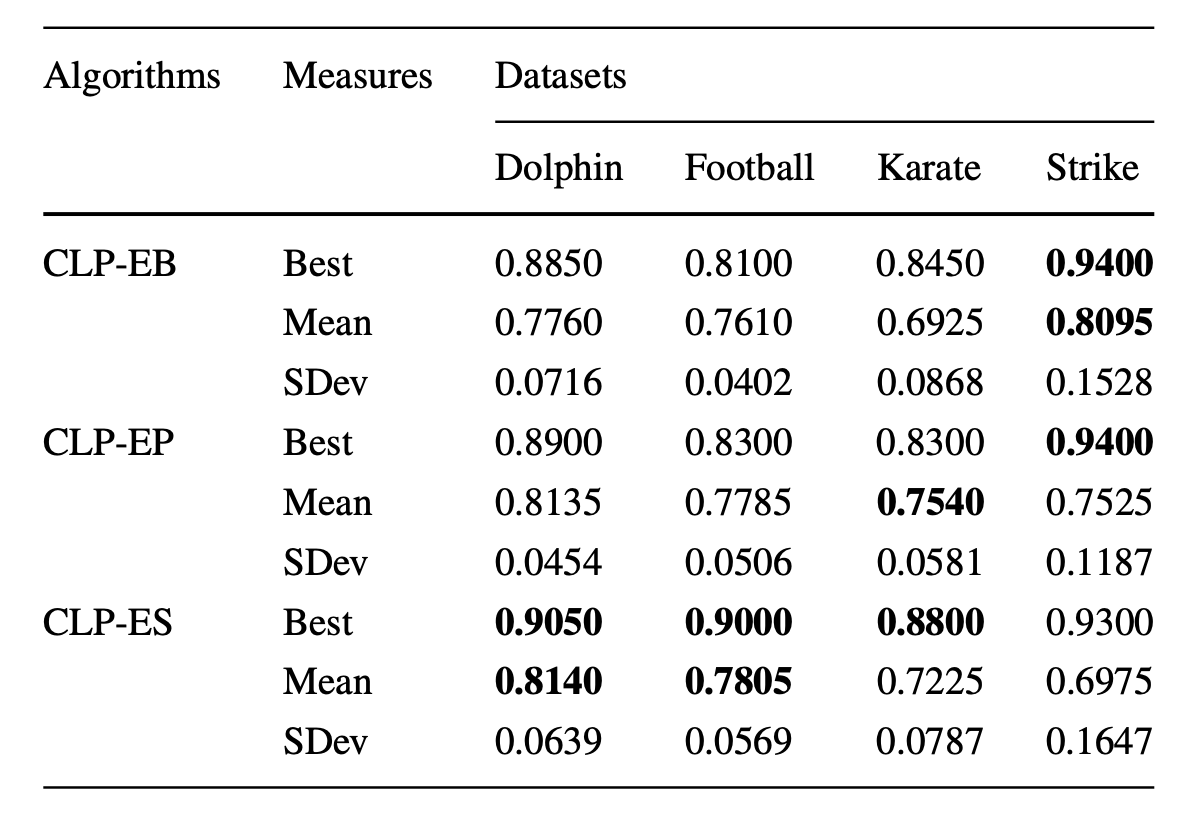
\includegraphics[width=6cm]{img/line_org.png}
  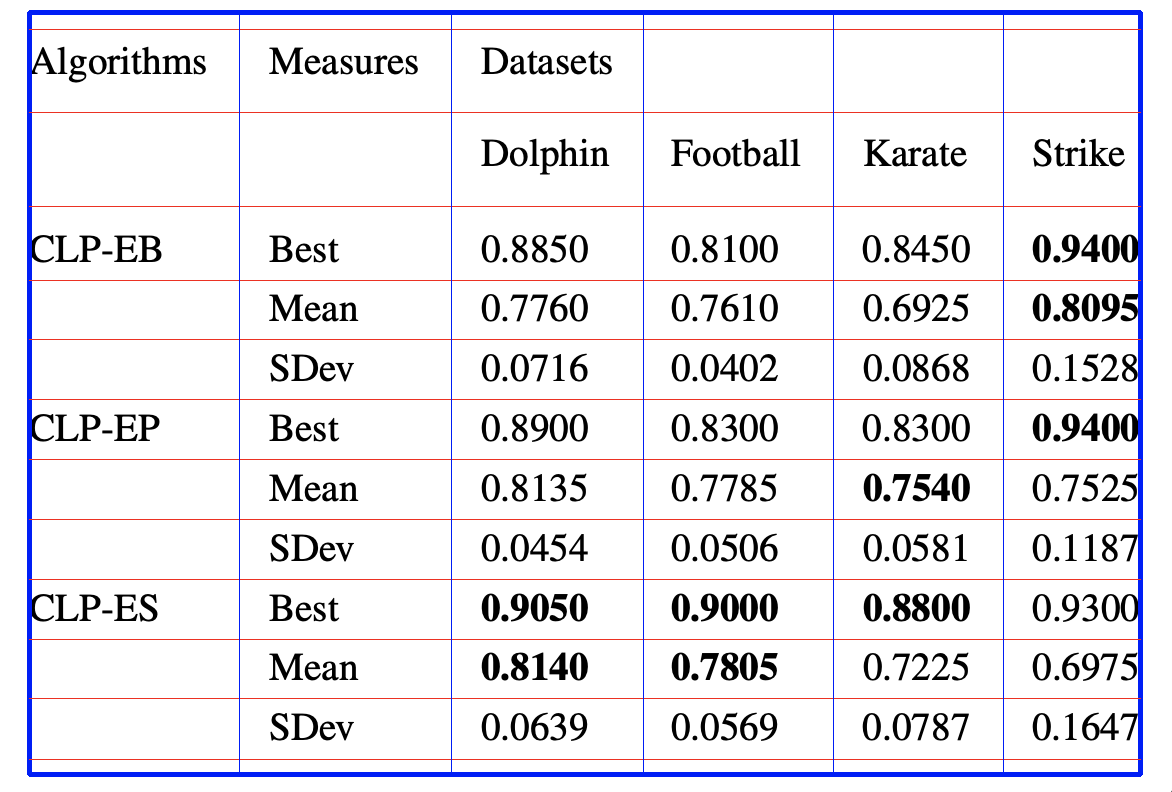
\includegraphics[width=6cm]{img/line.png}
  \caption{Example of Line Construction}
  \label{fig:line}
  \end{center}
\end{figure}

\paragraph{Remark} The implementation has been provided by the teaching assistant in \texttt{table\_reconstruction.py}. However, this implementation has a few limits, remarked as follows

\begin{itemize}
    \item In step \ref{step:extract}, the contour of the table has to be determined with the help of existing frames (e.g. the top frame and the bottom frame). In other words, this method will not work on a table without any frames. But this can happen since tables in real pdf files can have various formats.
    \item In step \ref{step:line}, the contour of the table is determined by the outmost point of line segments. Therefore, this method requires that the input should be an independent image instead of a whole page.
    \item In step \ref{step:draw}, the lines are drawn by scanning the whole row. However, some table may have joint headers, disabling the detection of some lines between columns, shown in Figure \ref{fig:line2}
\end{itemize}


\begin{figure}[ht]
    \begin{center}
    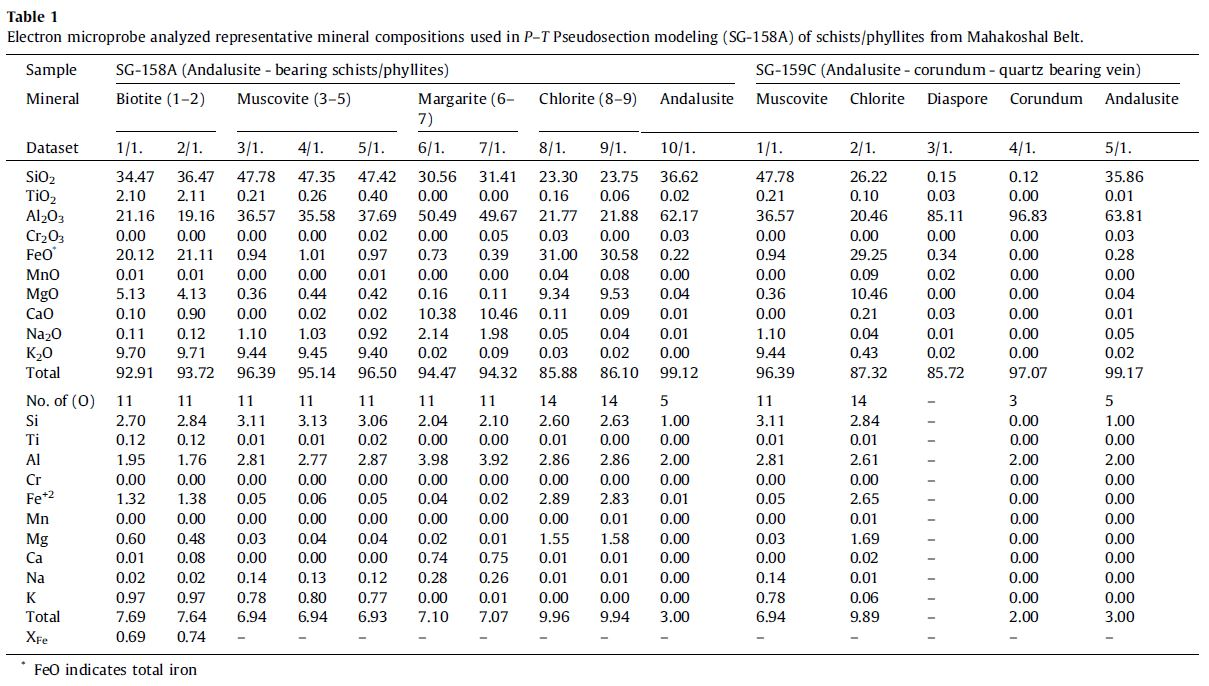
\includegraphics[width=6cm]{img/line1_org.JPG}
    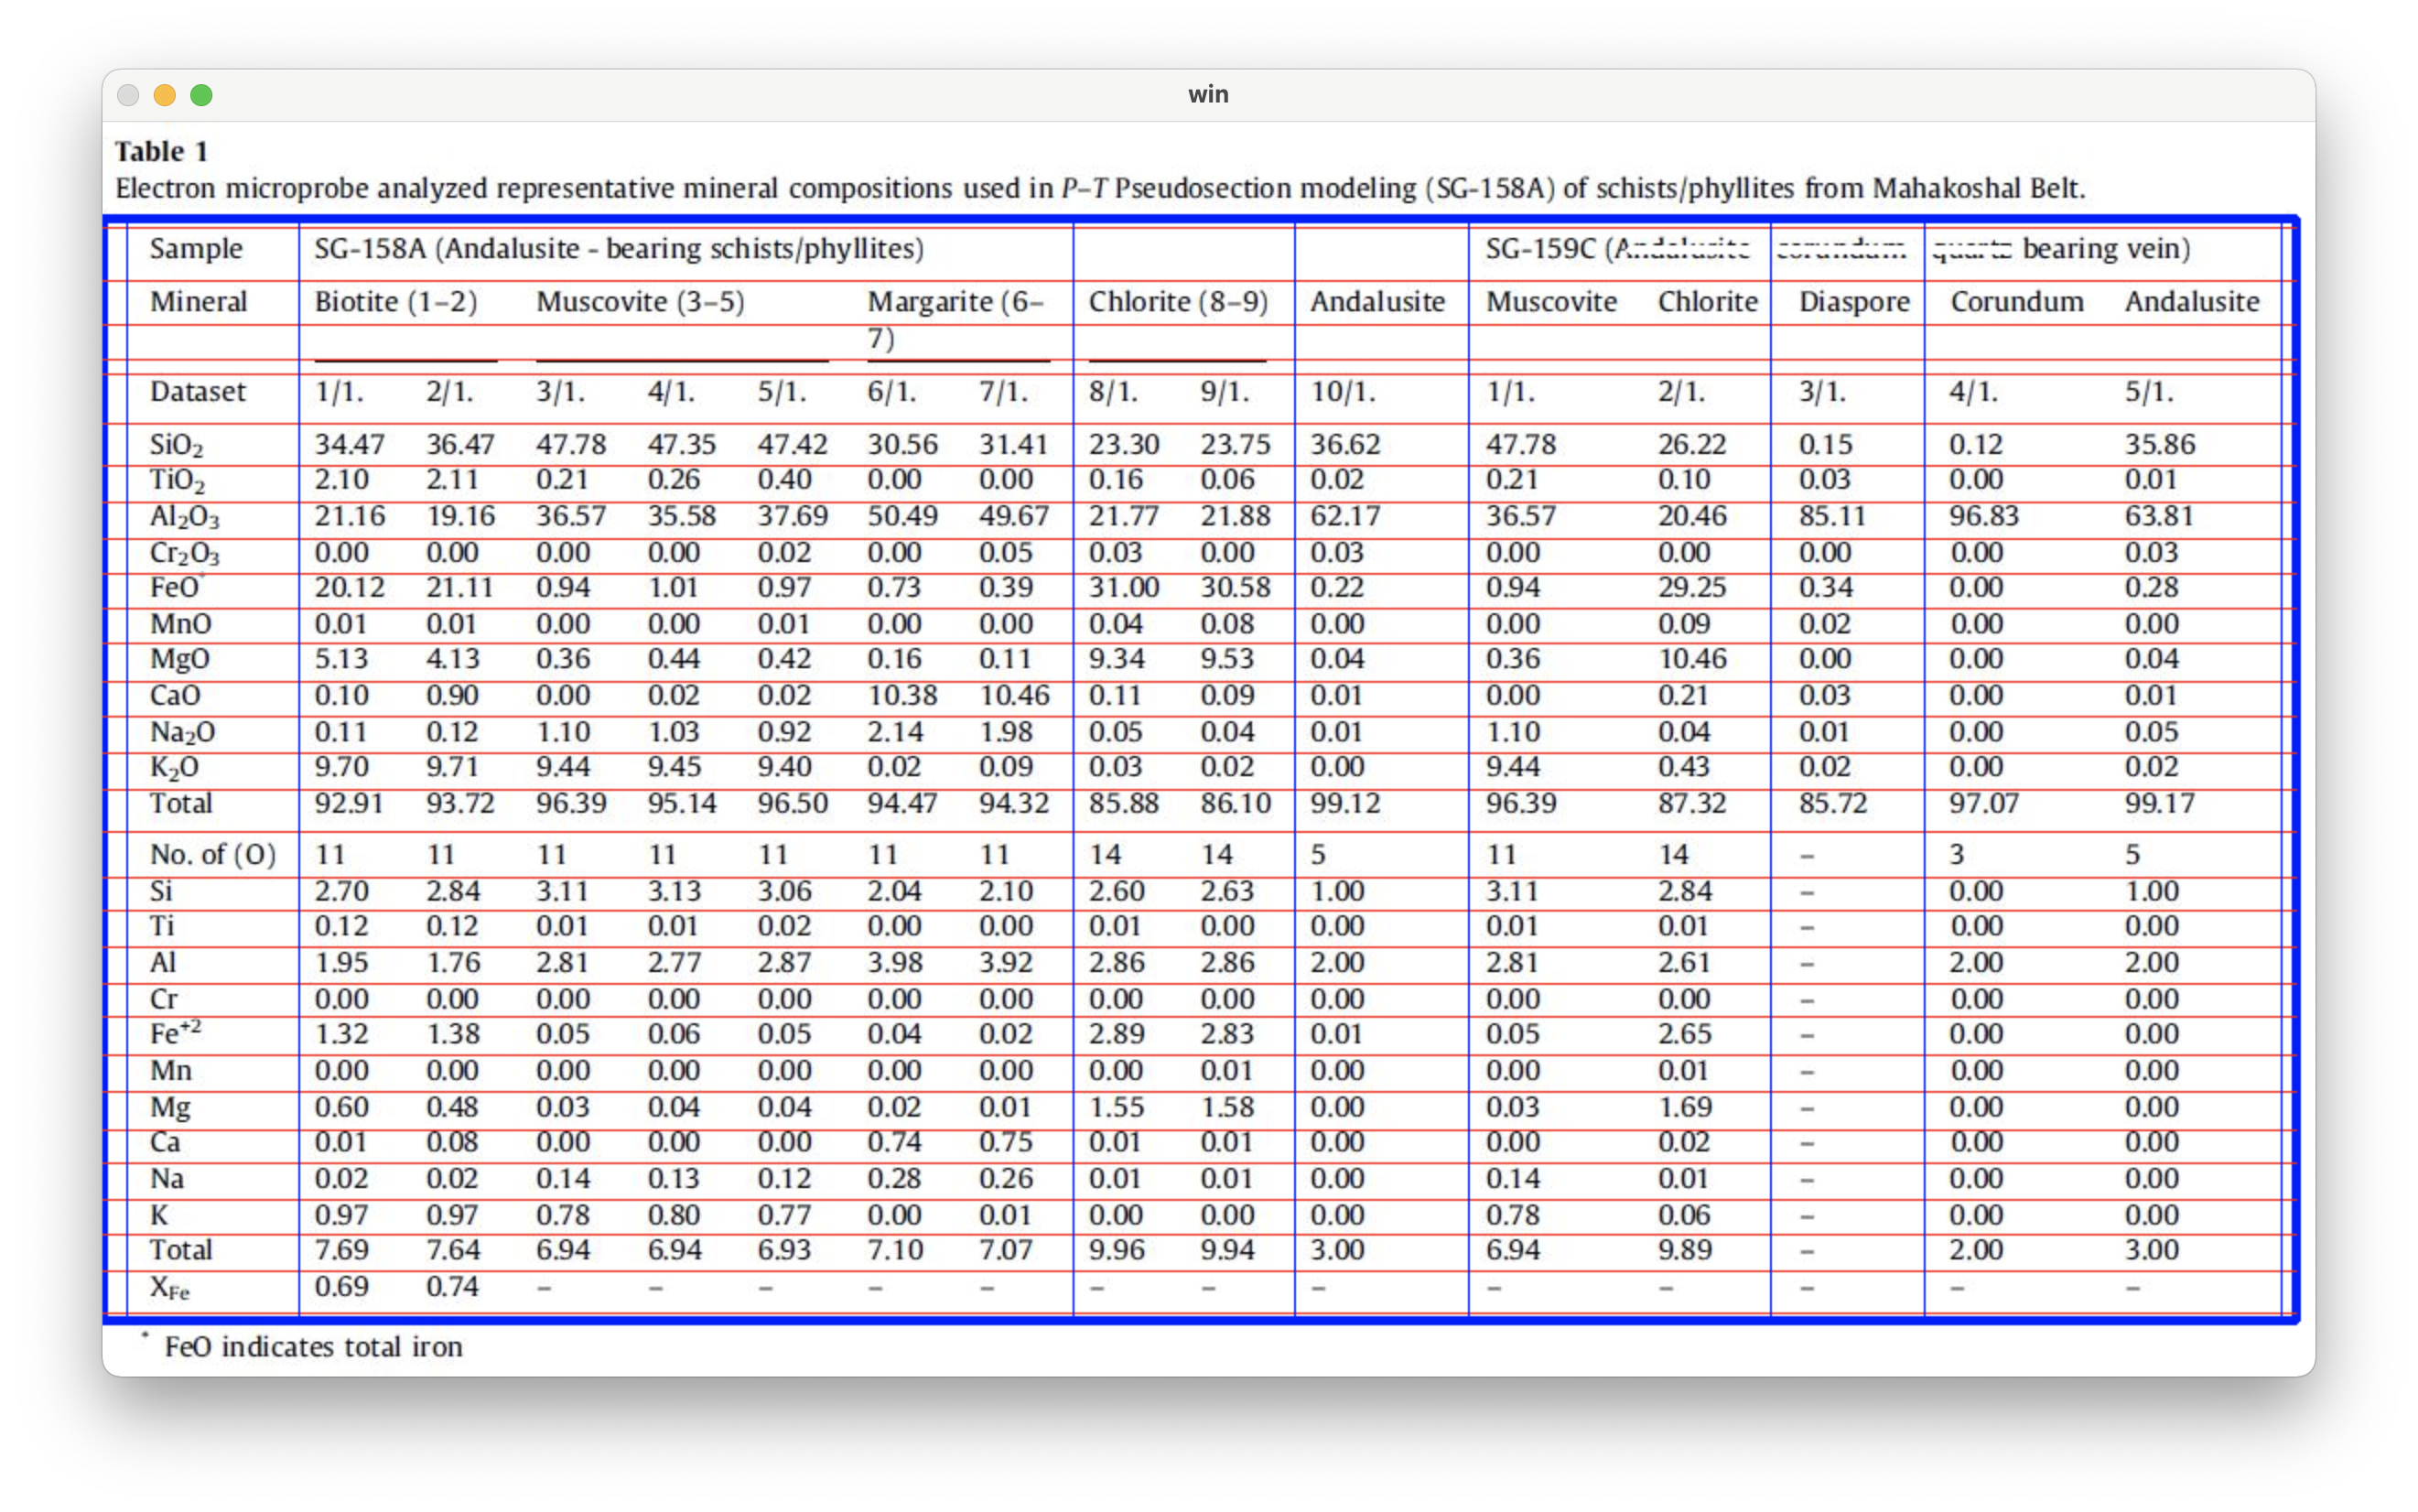
\includegraphics[width=6cm]{img/line1.png}
    \caption{Example of Line Construction}
    \label{fig:line2}
    \end{center}
  \end{figure}

\section{Table Detection}

The above problem mainly stem from the fact that the methods implemented in \texttt{table\_reconstruction.py} does not fully consider textual information, but relies on an outmost ``frame'' to locate the table.

To address this issue, we tried another method\footnote{Reference: \texttt{https://stackoverflow.com/questions/50829874/how-to-find-table-like-structure-in-image}} in \texttt{detect\_table.py}, which can not only reconstruct table lines, but also detect the table on a page with texts.

The steps of the methods are listed as follows.

\begin{enumerate}
    \item Use \texttt{cv2.dilate} to convert the text into the solid spots, shown in Figure \ref{fig:dilate}.
    \item Apply \texttt{cv2.findContours} to find text bounding boxes.
    \item Filter the bounding boxes within an appropriate height range (i.e. the height of a normal-sized font).
    \item Cluster the text boxes into groups by their coordinates, so that we can find a groups of text areas aligned into rows and columns.
    \item Sort them by x and y coordinates, find if the grouped text boxes can form a table.
\end{enumerate}


\begin{figure}[ht]
  \begin{center}
  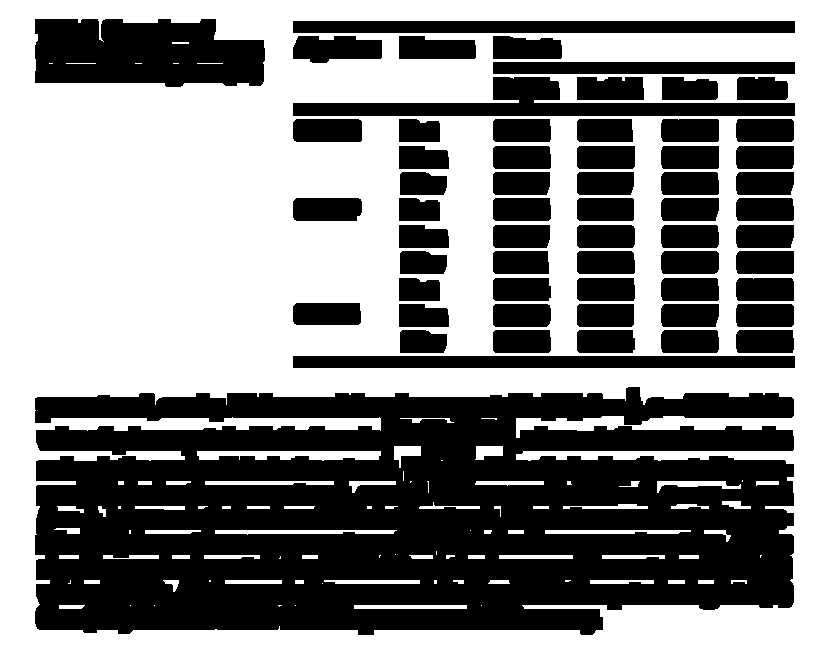
\includegraphics[width=12cm]{img/pre.png}
  \caption{Dilated table image}
  \label{fig:dilate}
  \end{center}
\end{figure}

The reconstructed image is shown in Figure \ref{fig:line3}

\begin{figure}[ht]
  \begin{center}
  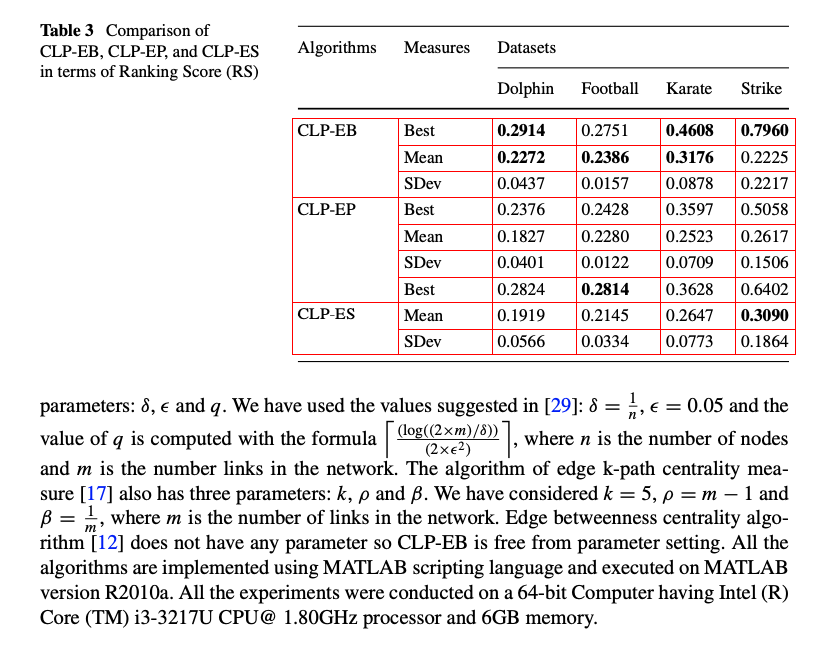
\includegraphics[width=12cm]{img/out.png}
  \caption{Image after table detection}
  \label{fig:line3}
  \end{center}
\end{figure}

The above method also serves as a solution to Exercise 1.

%%%%%%%%%%%%%%%%%%%%%%%%%%%%%%%%%%%%%%%%%%
%%%%%%%%%%%%%                 %%%%%%%%%%%%
%%%%%%%%%%%%%    EXERCISE 1   %%%%%%%%%%%%
%%%%%%%%%%%%%                 %%%%%%%%%%%%
%%%%%%%%%%%%%%%%%%%%%%%%%%%%%%%%%%%%%%%%%%
\begin{exercise}[]{How to automatically locate the tables in a PDF?}
  \begin{solution}
  \par{~}
  The main idea is that unlike texts, all table structures share a clear space separator for us to infer its table lines. To make it easier for us to analyze, we can first dilate the text areas, so that texts will be joined together but not for tables. We can then find contours on the image and group the boxes to detect if they form a whole table.
  \end{solution}
  \label{ex1}
\end{exercise}

%%%%%%%%%%%%%%%%%%%%%%%%%%%%%%%%%%%%%%%%%%
%%%%%%%%%%%%%                 %%%%%%%%%%%%
%%%%%%%%%%%%%    EXERCISE 2   %%%%%%%%%%%%
%%%%%%%%%%%%%                 %%%%%%%%%%%%
%%%%%%%%%%%%%%%%%%%%%%%%%%%%%%%%%%%%%%%%%%
\begin{exercise}[]{What do you think is the most difficult step to extract the table from the PDF? why?}
  \begin{solution}
  \par{~}
  In our new implementation, we will have to tune many parameters, such as dialating size, the range of the filtered boxes and the criteria for recognizing a table. In real world, the tables in different papers have different table formats and some tables may have nested structures. These parameters should be tuned carefully so that the method can achieve its generality. Some deep learning methods may help with this issue.
  \end{solution}
  \label{ex2}
\end{exercise}


\end{document}